\documentclass[11pt]{extarticle}
\usepackage{fullpage}
\usepackage[ampersand]{easylist}
\ListProperties(Hide=10, Style*=$\bullet\;\,$, Style2*=$\;\,${\tiny$\blacksquare$}$\;\,$,Space*=1mm,Space2*=0.1mm)

\usepackage{hyperref}
\hypersetup{colorlinks=true,
	linkcolor=black,
	filecolor=black,      
	urlcolor=black}

\usepackage{amsmath,amssymb,amsthm,mathtools,mathrsfs}
\newtheorem{thm}{Theorem}[]
\usepackage{bibref}

\usepackage[T1]{fontenc}
\usepackage[sc,osf]{mathpazo}
\usepackage{eulervm}
\usepackage[bold=.05]{xfakebold}

\usepackage{tikz}
\usetikzlibrary{calc}
\usetikzlibrary{shapes}
\usepackage{pgfplots}
\pgfplotsset{trig format plots=rad}
\usetikzlibrary {3d}
\pgfplotsset{compat=1.18}

\usepackage[most]{tcolorbox}
\tcbuselibrary{skins}
\usepackage[explicit]{titlesec}
\newtcolorbox{secbox}[1][]{enhanced,attach boxed title to top center,drop fuzzy shadow,breakable,colbacktitle=gray,colback=black,colframe=black,
	coltext=white,size=title,title={#1}}
\titleformat{\section}[runin]{\bfseries\LARGE}{}{0pt}{\hfill
	%\begin{secbox}[\thesection]
	%	\centering #1
	%\end{secbox}
	%}
\tcbsidebyside[sidebyside adapt=left,segmentation style=solid,enhanced,size=small]
{%
	\thesection 
}
{%
	#1
}
}
\titleformat{\subsection}[runin]{\bfseries\large}{}{0pt}
{\hfill
%	\begin{secbox}[\thesubsection]
	%		\centering #1
	%	\end{secbox}
\tcbsidebyside[sidebyside adapt=left,segmentation style=solid,enhanced,size=small]
{%
	\thesubsection 
}
{%
	#1
}
}
\titleformat{\subsubsection}[runin]{\bfseries}{}{0pt}
{\hfill
%		\begin{secbox}[\thesubsubsection]
	%			\centering #1
	%		\end{secbox}
\tcbsidebyside[sidebyside adapt=left,segmentation style=solid,enhanced,size=small]
{%
	\thesubsubsection 
}
{%
	#1
}
}

\usepackage{multicol}
\setlength{\columnsep}{5mm}
\setlength\columnseprule{.1pt}

\newcommand{\ra}{\rightarrow}
\newcommand{\R}{\mathbb{R}}
\newcommand{\C}{\mathbb{C}}
\newcommand{\Na}{\mathbb{N}}
\newcommand{\Z}{\mathbb{Z}}
\newcommand{\Q}{\mathbb{Q}}
\newcommand{\w}[1]{\text{#1}}
\newcommand{\ck}{.\,.\,}
\newcommand{\sm}[2]{\displaystyle\sum_{#1}^{#2}}
\newcommand{\Uint}[2]{\overline{\int\!}_{#1}^{\;#2}}
\newcommand{\Lint}[2]{\underline{\int\!}_{\;#1}^{\;#2}}
\newcommand{\pfrac}[2]{\frac{\partial#1}{\partial#2}}
\newcommand{\ckfil}{$.\dotfill.$}
\newcommand{\tm}{\times}
\newcommand{\snote}[1]{{\footnotesize(#1)}}
\newcommand{\st}{\,{}_{s}|_t\,}
\newcommand{\gen}[1]{\langle #1 \rangle}
\newcommand{\tbx}[2][]{
	\begin{tcolorbox}[enhanced,breakable,size=small,colback=black!2!white,title={#1},arc is angular, arc=1.5mm,drop fuzzy shadow]
		#2
	\end{tcolorbox}
}
\newcommand{\y}{$\blacksquare\;$}
\author{Yashas.N}
\title{Abstract Algebra : Ring Theory.}
\date{}
\begin{document}
	\maketitle
	\begin{multicols}{2}
			\section*{symbols used}
		\begin{center}
			$ \st \, \ra  $ such that.\\
			
		\end{center}
		\section{Basic Definitions}
			\tbx{ \textbf{Ring } $R$ : is a set together with two binary operations $ + $ and $ \tm $ \snote{addition  and multiplication} with properties :\\
			\y $ (R,+) $ is an abelian group \\
			\y $ \tm $ is associative \snote{ i.e. $ a\tm (b \tm c)=(a\tm b)\tm c  $} \\
			\y $ \tm $ distributes over $ + $ \snote{i.e. $(a+b)\tm c= (a\tm c)+(b\tm c)$}.} 

\tbx{if $ R $ is commutative w.r.t. $ \tm $ then $ R $ is a \textbf{Commutative ring}.
			} 
\tbx{Additive identity in $ R $ is denoted by $ 0 .$
			} 
\tbx{$ R $ is said to have identity $ (1) $ if there is a multiplicative identity  in $ R $ \\
			i.e. $\exists 1\in R  \st  1\tm a= a\tm 1=a\; \forall a\in R. $ 
			} 
\tbx{now for $ a\in R $ additive inverse of $ a $ is denoted by $ -a $ and multiplicative inverse \snote{if exists in $ R $} by $ a^{-1}.$
			} 
\tbx[\textbf{Division Ring} \snote{ or skew field} $ D $  ]{is ring with identity $ 1 $, $ 1\neq 0 $  and   for  a element $ a\in R $ not equal to $ 0 $ there exists $ b \in R \st ab=ba=1.$ i.e. $ \forall 0 \neq  a \in R \, a^{-1}\in R.$ 
			} 
\tbx{for a ring $ R $ is a non zero $ a\in R $ is a \textbf{Zero Divisor} if there is non zero $ b\in R $ such that 
			$ ab=0 $ or $ ba=0. $
			} 
\tbx{for a ring $ R $ with $ 1 $ : $ u \in R $ is a \textbf{unit} in $ R $ if it has multiplicative inverse in $ R $
			} 
\tbx[\textbf{Integral domain} $ I $  ]{ is a commutative ring with identity $ 1\neq 0 $ having no zero divisors.
			} 
\tbx[\textbf{Field } $ F $ ]{is a commutative ring with identity in which any non zero element is unit i.e. 
			$ 0\neq a \in F\implies a^{-1} \in F.$ or a commutative Division ring.
			} 
\tbx{\textbf{Subring }S of ring $ R $ is subgroup of $ R $ which is in itself a ring with same operations i.e. $ S $ is subring of $ R $ if $ (S,+) $ is subgroup of $ (R,+) $ and $ S $ is closed under $ \tm .$ \\
			\snote{i.e. $ a,b\in S \implies ab \in S $}
			} 
\tbx{\textbf{Center} of a ring $ R $ is set $ \{ z\in R \st zr=rz \forall r\in R\} $ i.e. all the elements that commute in $ R. $ (multiplicatively.)
			} 
\tbx{$ a \in R $ commutative ring is \textbf{nilpotent} if $ a^m=0 $ for some $ m \in \Z^+ $}
\tbx{$ a \in R $ commutative ring is \textbf{idempotent} if $ a^2=a $.}
		\section{Properties of Rings}
		\snote{instead of writing $ a\tm b $ we just write $ ab $}
		
\tbx{for any $ a,b \in R $ (ring)\\
			\y $ a0=0a=0 .$ \\
			\y $ (-a)b=a(-b)=-(ab). $ \\
			\y $ (-a)(-b)=ab $ \\
			\y if $ 1\in R $ then $ -a=(-1)a. $ \\
			} 
\tbx{An element cannot be both a zero divisor and a unit in $ R .$ \snote{ There can be elements that are neither}
			} 
\tbx{if $ ab=0 $ in a integral domain $ I $ with $ a,b \in I $ then at least on of $ a $ or $ b $ is zero.
			} 
\tbx{Cancellation Laws holds in any Integral domain. \snote{note: the existence of multiplicative inverse is not needed here.}
			} 
\tbx{\textbf{Any Finite Integral Domain is a Field} \\
			\snote{use bijective map $ I \ra I \w{ by } x\ra ax $ for non-zero $ a \in I.$}
			} 
\tbx{if $S,T $ subgrings of $ R $ then :\\
	\y $ S\cap T $ is subring of $ R .$ \snote{ thus any arbitrary non-empty intersection of subrings is a subring.}\\
   \y $ S $ is subring of $ T $ is subring of $ R $ then $ S $ is subring of $ R. $
			} 
\tbx[Properties of Center of a Ring]{
	\y Center of a ring is a subring.\\
\y Center of a Division ring is a Field.\\	
\y for fixed $ a\in R $ set $ C(a) =\{r\in R \st ra=ar\}$ is a subring of $ R $ containing $ a. $ \\
\y Center of $ R $ $ = \underset{a\in R}{\cap}{C(a)}. $\\
\y for any $ a\in D $ division ring then $ C(a) $ is a division ring.
			} 
\tbx{if $ x^2=1 $ for some $ x\in I $ integral domain then $ x=\pm 1 $ only.
			} 
\tbx{if $ x\in R $ commutative ring is nilpotent then\\
			\y $ x $ is either zero or zero divisor  
			\snote{use $ x^m=x^{m-1}x=0 $}\\
			\y $ rx $ is nilpotent for any $ r\in R. $ \\
			\y if $ 1\in R $ then $ 1+x $ is a unit in more general $ u+x $ is a unit for any unit $ u $ and nilpotent $ x .$
			\snote{ use $ (1+x)(1-x+x^2+\ck + (-1)^{m-1}x^{m-1})=1+(-1)^{m-1}x^m=1 $.}\\
			} 
\tbx{for rings $R  $ and $ S $ their direct product $ R\tm S $ is ring under corresponding component wise operation. \snote{ thus even any number of direct product of rings is a ring }
			} 
	\tbx{now if $ R,S $ are non zero fields then $ R\tm S $ is never a field. \snote{as $ (1,0)(0,1)=(0,0) $}}
\tbx[\textbf{Characteristic } $ ch(R) $  ]{Characteristic  of a ring is a number \\
			$ n \st n1=\overbrace{1+1+\ck +1}^{n \w{ times }}=0$ if order of $ 1 $ is infinite then characteristic is said to be $ 0 $ \snote{ not $ \infty $.}
			} 
\tbx{\textbf{every Integral domain has a Character $ 0 $ or prime.} \snote{if  $ q=mn $ is characteristic of $ I $ then $ mn.1=0 $ so either $ m.1=0 $ or $ n.1=0 $ a contradiction for minimality.}}
		\section{Ring Homomorphism and Ideals}
		
\tbx{if $ R,S $ are two rings the a map $ \phi :R \ra S $ is a ring Homomorphism if it satisfies
			\y $ \phi(a+b)=\phi(a)+\phi(b) $ \\
			\y $ \phi(ab)=\phi(a)\phi(b) $ \\
			} 
\tbx{\y kernel of $ \phi  $ denoted by ker $\phi $ is the set in $ R $ mapped to $ o $ in $ S $
\\
\y image of $ \phi $ and ker $\phi  $ are subrings.\\
\y if $\alpha\in   $ ker $ \phi $ then $ r\alpha \in  $ ker $ \phi $ $ \forall r \in R $\\
			i.e. $ r $ ker $ \phi \subseteq  $ ker $ \phi $
			} 
\tbx[Concept of Ideal]{From the above point and to define the quotient operations as in group homomorphism i.e. if  $ I \subseteq R $ and to the quotient operations 
			\begin{center}
				$ (r+I)+(s+I)=(r+s)+I $\\
				$ (r+I)(s+I)=rs+I $
			\end{center}
			to be well defined we need to have that replacement by any class representative gives same classes i.e.
			if $ \alpha, \beta \in I $ then \\
			$ (r+\alpha)(s+\beta)+I=rs+I $\\
			to achive this : we need $ I \trianglelefteq R $ (w.r.t $ + $) this can be satisfied by any subgroup of $ R $ as $ R $ is abelian in $ + $, letting $ r=s=0 $ we need $ I $ closed under multiplication so these two conditions boils down to $ I $ must be subring of $ R $ 
			and also we need to have that $ I $ must be closed under left and right multiplication from any element in $ R $
			i.e. $ rI \subseteq I, Ir\subseteq I \; \forall r\in R $ this leads us to define Ideals
			} 
\tbx{$I \subseteq R  $ is a \textbf{left ideal} in $ R $ if $ I $ is subring of $ R $ and closed under left multiplications by elements of $ R $, similarly $I \subseteq R  $ is a \textbf{right ideal} in $ R $ if $ I $ is subring of $ R $ and closed under right multiplications by elements of $ R $.\\
			Finally $ I \subseteq R $ is an \textbf{Ideal }of $ R $ if it is both left and right ideal of $ R $
			} 
\tbx{Ideal for Rings is `similar' to Normal subgroups for Groups, Most of the following properties are Ring analogue of Group properties.
			} 
\tbx{ if $ I $ is an ideal of $ R $ ring then the quotient group (additive $ \{r+I\} $) is a ring with binary operations as defined above. This Group $ R/I $ is called the \textbf{Quotient ring} of $ R $ by $ I. $
			} 
\tbx[\textbf{Isomorphism Theorems for Ring}]{
			\y \textbf{1st Isomorphism Theorems for Ring} : \\ 
			if $ \phi : R\ra S $ is a ring homomorphism then ker $ \phi $ is an ideal of $ R $, image of $ \phi $ in $ S $ is a subring of $ S $ and $ R/ker(\phi) $ is isomorphic (bijective ring homomorphism) to $ \phi(R) .$ let $ \cong $ denote Ring isomorphism from here on so $ R/ker(\phi)\cong \phi(R) $\\
			if $ I $ is an ideal of $ R $ then the natural projection homomorphism $ \pi_I:R \ra R/I $ by $ \pi_I(r)=r+I $ is ring homomorphism   with kernel $ I $ i.e. ideal $ \iff $ kernel.\\
			\y  \textbf{2st Isomorphism Theorems for Ring} : \\ 
			If $ A $ is subring of $ R $ and $ B $ ideal of  $ R $ then $ A+B=\{a+b|a\in A,b\in B\} $ is a subring of $ R $, $ A\cap B $ is an ideal of $ A $ and $ (A+B)/B\cong A/(A\cap B) .$\\
			\y  \textbf{3st Isomorphism Theorems for Ring} : \\ 
			if $ I,J $ are ideals of $ R $ such that $ I	\subset J $ then $ J/I $ is an ideal of $ R/I $ and $ (R/I)/(J/I)\cong R/J $\\
			\y \textbf{4st Isomorphism Theorems for Ring} :  \\
			If $ I $ is an Ideal of $ R $ ring then the map $ A\ra A/I $ is bijective between the set of subrings $ A $ of $ R $ that contain $ I $ and set of subrings of $ R/I $ also $ A $ is an ideal of $ R $ containing $ I $ iff $ A/I $ is an ideal of $ R/I .$
			} 
\tbx{if $ \phi : R \ra S $ is homomorphism and $ x	\in  R$ is nilpotent then $ \phi(x) $ is nilpotent in $ S. $}
			\subsection{Properties of ideal}
			\textbf{\large \emph{Let $ R $ be a ring with identity for this subsection.}}
			
\tbx{for ideals $ I,J $ of $ R $ ring define $ I+J=\{a+b|a\in I,b\in J\} $ and $ IJ= \gen{ab|a\in I,b\in J} $ \snote{i.e. the set generated by $ ab $ or set of finite sums of element of form $ ab $} then\\
			$ I+J $ is the smallest ideal containing both $ I $ and $ J $ in $ R, $\\
			$ IJ \subset I \cap J $ and both $ IJ , I\cap J$  are ideals in $ R. $\\
			} 
\tbx{\textbf{Ideal Generated} by $ A  \subseteq R $ denoted by $ (A) $ is the smallest ideal of $ R $ ring containing $ A .$
			} 
\tbx{define $ RA=\{r_1a_1+r_2a_2+\ck +r_na_n| r_i\in R, a_i\in A\} $ and $ AR=\{a_1r_1+a_2+r_2a_2+\ck +a_nr_n|a_i\in A, r_i\in A\} $ and $ RAR= \{r_1a_1r'_1+r_2a_2r'_2+\ck +r_na_nr'_n| r_i,r'_i\in R, a_i\in A\}$
			} 
\tbx{if $ R $ is commutative then $ RAR=RA=AR=(A) .$
			} 
\tbx[Principle Ideal]{An ideal generated by a single element is called a Principle Ideal,\\
			An ideal generated by a finite set is called \textbf{Finitely generated ideal.}
			} 
\tbx{$ I$ is an ideal of $ R $ ring and $ I=R $ iff $ I  $ contains an unit of $ R .$\\
So we get $ R $ is a field iff the only ideals of $ R $ are $ \{0\} $ and $ R. $
			} 
\tbx{if $ F $ is field then any homomorphism from $ F $ is trivial \snote{$ ker(\phi)=F$} or injective 
			\snote{$ ker(\phi) = 0$} i.e. \textbf{any non trivial homomorphism from a field is injective}
			} 
\tbx[\textbf{Maximal Ideal}]{$ M $ a proper ideal of $ R $ ring is called a Maximal  Ideal of $ R $ if the only ideal containing $ M $ in $ R $ is $R. $ i.e. no other proper ideals contains $ M $ in $ R. $
			} 
\tbx{$ M $ is maximal ideal of $ R $ ring iff $ R/M $ is a field.
			} 
\tbx{\textbf{for a Ring with identity every proper ideal is contained in a maximal ideal} \\
			\snote{ inclusion forms a partial ordering of proper ideals (non empty set) in the ring so a chain exist whose elements always contain the given proper ideal, now form an ideal by union of these ideals which is also proper (prove) thus a having upper bound and by Zorn's lemma a maximal element which is the maximal ideal.}
			} 
\tbx[\textbf{Prime ideal }]{An ideal $ P $ is Prime Ideal of $ R $ ring if $ P\neq R $ and whenever $ ab\in R $ the $ a\in P $ or $ b\in P .$\\
			\snote{this is sort of generalising `prime' to a give ring $ R $ as in $ \Z^+ $ if $ p $ is a prime and 
				$ p|ab $ then $ p|a $ or $ p|b. $} 
			} 
\tbx{for $R  $ a commutative ring $ P $ is prime ideal in $ R $ iff  $ R/P $ is an Integral domain.
			} 
\tbx{from above point and similar point for maximal ideals we get : \\
			\textbf{in commutative ring $ R $ every maximal ideal is a prime ideal}
			} 
\tbx{similarly a commutative ring with identity is an integral domain iff $ \{0\} $ is prime ideal in the ring.
			} 
\tbx{in an Integral domain $ R $ $ (a)=(b) $ for some $ a,b \in R $ iff  $ a=ub $ for some unit $ u\in R .$
			} 
\tbx{if $ P $ a prime ideal of $ R $ commutative ring and $ P $ contains no zero divisors then $ R $ is an integral domain. 
			} 
\tbx{if $ \phi : R \ra S $ be a ring homomorphism between two commutative rings with identity:\\
			\y for $P $ prime ideal in $ S $ then $ \phi^{-1}(P) $ is a prime ideal in $ R $ or $ \phi^{-1}(P)=R $ \\
			\y if $ \phi $ is \textbf{surjective} and $ M $ maximal ideal in $ S$ then $ \phi^{-1}(M) $ is maximal in $ R. $ \\
			} 
\tbx{\textbf{In a finite commutative ring with identity every prime ideal is maximal ideal}.\\
			\snote{use finite integral domain is a field.}
			} 
\tbx{if $R$ is commutative ring with property : for every $a\in R \; \exists n\in \Z^+${ depending on }$a \st a^n=a$ then every prime ideal of $ R $ is maximal idea.}

		\section{Ring of fractions} 

\tbx{let $ R $ be a commutative ring and $ \{0\}\neq D\subseteq R $ that doesn't contain $ 0 $, doesn't contain any zero divisors of $ R $, closed under multiplication then there is a commutative ring $ Q $ with $ 1 $ such that 
			$ R $ is a subring of $  Q$ and every element of $ D $ in $ Q $ has an inverse.\\
			This ring $ Q $ has  following additional properties :\\
			\y every element of $ Q $ is of the form $ rd^{-1} $ for some $ r\in R, d\in D $ in particular If 
			$ D=R-\{0\} $ then $ Q $ is a field.\\
			\y Ring $ Q $ is the smallest ring containing $ R $ in which all elements of $ D $ are units \\
			\snote{i.e. if $ \phi : R\ra S $ is an injective homomorphism $ \st $ $ \phi(d) $ is a unit in 
				$ S $ then there is An isomorphic copy of $ Q $ in $ S .$}\\
			this $ Q $ is called the \textbf{Ring of Fractions.} of $ D $ w.r.t $ R. $
			} 
\tbx[Construction of Ring of fractions ]{
			let $ \mathcal{ F} = \{ (r,d) \st r\in R, d\in D \}$ and define relation $ \sim $ on 
			$ \mathcal{ F} $ by $ (r,d)\sim (s,e) $ iff $ re=sd $ this becomes an equivalence relation as 
			$d,e$ are not zero divisors, denote equivalence class of $ (r,d) $ by 
			\begin{center}
				$\frac{ r}{  d}=\{ (a,b)\st a\in R, b\in D \w{ and } rb=ad\} $ 
			\end{center}
			then $ Q $ becomes the set of equivalence classes under $ \sim $ \\
			properties such as commutativity , $1= \frac{ d}{d  }$, additive inverse of $ \frac{ a}{  d} $
			is $ \frac{ -a}{  d} $, $ d^{-1}= \frac{ 1}{  d} \; \forall d\in D$ hold making this $ Q $ the 
			ring of fractions.
			} 
\tbx{$ Q $ may also be denoted by $ D^{-1}R $ to emphasize the envolved $ R,D .$\\
If $ R $ is integral domain and $ D=R-\{0\} $ then $ D^{-1}R $ is a field so is called 
			\textbf{ Field of Fractions} of $ R .$\\
If $ R$ is an integral domain, $ Q $ its field of fractions then if any field $ F $ contains
			$ R' \st R'\cong R $ then the subfield generated by $ R' $ in $ F $ is isomorphic to $ Q. $
			} 
\tbx{This concept of integral domains and field of fractions are derived from observing $ \Z,\Q $
			this is generalized by\\
			if $ F $ is Field then $ F $ contains a unique smallest subfield that is either isomorphic to 
			$Q $ or $ \Z/p\Z .$ \snote{ depending on its characteristic.}}
			
	
		
		\section{Euclidean Domain.}

\tbx[\textbf{Norm} $ N $]{Norm $ N $ on $ R $ integral domain is a function from $ R\ra Z^+\cup \{0\} $ with $ N(0)=0. $\\
			if $ N(a)>0 $ for $ a\neq 0 $ in $ R $ then $ N $ is called\textbf{ positive norm .}
			} 
\tbx{for $ R $ an integral domain is called an \textbf{Euclidean Domain} if there is a norm $ N $ on $ R $ such for any $ a,b\in R $ with $ b \neq 0$ there exist elements $ q,r\in R $ such that 
			\begin{center}
				$ a=qb+r $ with $ r=0 $ or $ N(r)<N(b) $
			\end{center} here $ q $ is called quotient and $ r $ the remainder of the division.
			} 
\tbx{Euclidean Division algorithm is valid in an Euclidean Domain \snote{i.e. it stops after finite steps.}
			} 
\tbx{Every ideal in Euclidean Domain is principal \snote{i.e. generated by single element that has the minimum norm.}
			} 
\tbx{in a commutative ring $ R $, $ a,b\in R $ and $ b\neq 0$
			\y $ a $ is said to be multiple of $ b $ if there exist $ x\in R \st a=bx. $ denoted by $ b|a $ \\
			\y \textbf{Greatest common divisor } of $ a,b\in R $ is a non zero $ d \in R \st  $ 
			$ d|a,d|b $ and if any other $ d'|a,d'|b $ then $ d'|d $\\
			this is denoted by $ (a,b)=d .$
			} 
\tbx[Properties of Gcd]
{\y if $ a,b \in R $ not zero , ideal generated by $ a,b $ is principal and equal to $ (d) $ then $ (a,b)=d $
			\snote{ literally $ (a,b)=(d) $ }\\
\y now $ (a,b)=d $ in $ R $ if $ I $ ideal generated by $ a,b $ is contained in $ (d) $ and any principle ideal $ (d') $ contains $ I \implies (d)\subseteq (d')$\\
\y as $ (d)=(d') $ then $ d=ud' $ for some unit $ u\in R $ Integral domain we have :\\
			in an Integral domain $ R $ if $ d',d $ are both g.c.d of $ a,b $ then $ d=ud' $ for some unit $ u\in R .$
\y if $ R $ is an Euclidean domain if $ (a,b) =d$ in $ R $ then $ d=r_n $ the last remainder in euclidean algorithm applied to $ a,b $ in $ R $ and $ d=xa+yb $ for $ x,y\in R .$
			} 
\tbx[\textbf{Universal side divisor}]{$ u\in  R$ is Universal side divisor if  for every $x\in R  $ there is some $ z\in R^*\cup \{0\} $ 
			\snote{ set of units in $ R $ + $ \{0\} $} such that $ u|(x-z). $ i.e every $ x $ can be written as $ x=qu+z. $ for $ z $ unit or zero.
			} 
\tbx[Test for not Euclidean domain]{If $ R $ is an integral domain which is not a field , $ R $ is a Euclidean domain then there is a universal side divisor in $ R $ \\
			\snote{this point can be used to disprove a given ring is euclidean domain.}}
		
		\section{Principal Ideal \\ Domains}

\tbx{\textbf{Principle ideal Domain} is an Integral domain in which every ideal is principal.
			} 
\tbx{Every Euclidean domain is a principal ideal domain.
			} 
\tbx{if $ R $ is a P.I.D. (Principal Ideal Domains) , $ (a,b)=d $ in $ R $ then $ d=xa+by $ for $ x,y\in R $ and $ d $ is unique upto multiplication by a unit in $ R .$
			} 
\tbx{\textbf{Every non zero prime ideal of a P.I.D. is a maximal ideal}
			} 
\tbx[\textbf{Dedekind-Hasse Norm}]{is positive norm on integral domain$ R $ 
			such that for every non zero $ a,b\in R $ either 
			$ a\in (b) $ or there exist a non zero element of ideal $ (a,b) $ which has a norm strictly smaller than norm of
			$ b $ i.e. $ \exists s,t\in R \st 0<N(sa-tb)<N(b) .$
			} 
\tbx[test for not a P.I.D]{Integral domain $ R $ is a P.I.D. iff $ R $ has a Dedekind-Hasse Norm.
			} 
\tbx{if $ R $ is an Integral domain in which every prime ideal is principal then $ R $ is a P.I.D.}
			
		\section{Unique Factorization Domain}

\tbx[Irreducible and prime]{For an Integral domain $ R $ :\\
			\y $ r\in R $ a non-zero non-unit element is called \textbf{irreducible} in $ R $ if whenever $ r=ab. $ with  $ a,b\in R $ \\
			then at least one of $ a,b $ is a unit in $ R $ \snote{ i.e. $ r $ cannot be factored into only non units}\\
			otherwise $ r $ is said to be \textbf{reducible}.\\
			\y non zero $ p \in R$ is called \textbf{prime} in $ R $ if $ (p) $ is a prime ideal in $ R. $ \\
			\snote{ i.e. if $ ab\in (p) $ then $ p|ab $ so $ p|a $ or $ p|b$ analogous to definition of `primes' in $ \Z $.}\\
			\y two elements $ a,b \in R $ are called \textbf{associates } in $ R $ if the differ by a unit in $ R $ i.e $ a=ub $ for some unit $u\in R  $ \\
			} 
\tbx{\textbf{In an integral domain every prime is irreducible.}
			} 
\tbx{\textbf{In a P.I.D. every non zero element is prime iff irreducible.}
			} 
\tbx{\textbf{U.F.D. (Unique Factorization Domain)} : is an integral domain in which every non zero element which is not a unit can be written as finite product of irreducibles and this decomposition is unique upto associates.
			\snote{i.e. for every non zero non unit $  r\in R$, $ r=p_ip_2\ck p_n $ for $ p_i's $ irreducibles and if same $ r=q_1q_2\ck q_m $ for $ q_i $ irreducible then $ m=n $ and we can rearrange these decompositions such that $ p_i,q_i $  are associates .}
			} 
\tbx{\textbf{In a U.I.D. every non zero element is prime iff irreducible.}
			} 
\tbx{if $ a,b\in R $ a U.I.D are such that $ a=up_1^{e_1}p_2^{e_2}\ck p_n^{e_n} $ and $ b=vp_1^{f_1}p_2^{f_2}\ck p_n^{f_n} $ for $ u,v $ units and $ p_i's $ primes in $ R $ then
			\begin{align*}
				(a,b)&=d\\
				&=p_1^{\min (e_1,f_1)} p_2^{\min (e_2,f_2)}\ck p_n^{\min (e_n,f_n)}.
			\end{align*}
			} 
\tbx{\textbf{Every P.I.D. is a U.I.D. in particularly every Euclidean Domain is a U.I.D.}
			} 
\tbx[\textbf{Fundamental theorem of Arithmetic}]{$ \Z $ is U.F.D.}

	\begin{flushleft}
		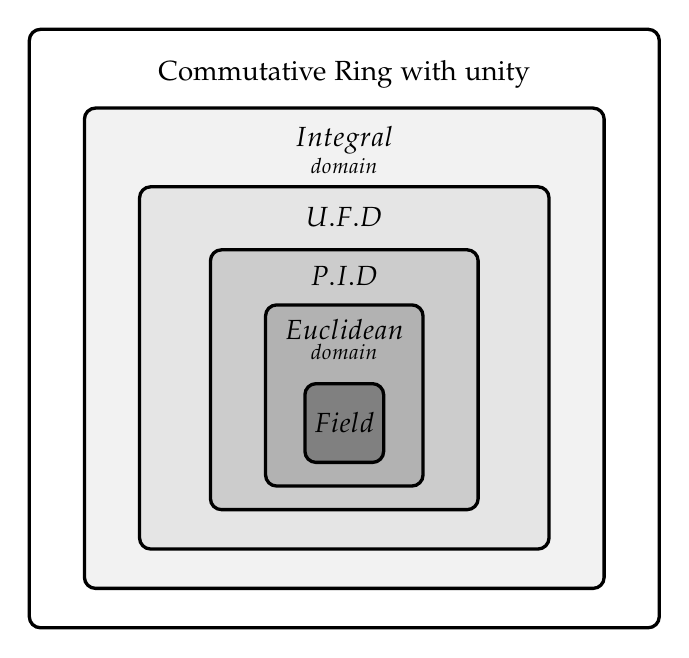
\begin{tikzpicture}
			\draw[very thick,rounded corners] (-4,5) rectangle node [above=83] {Commutative Ring with unity}(4,-2.6) ;
			\draw[very thick, ,fill=black!5!white,rounded corners] (-3.3,4) rectangle node [above =58] {$\underset{domain}{Integral}$}(3.3,-2.1) ;
			\draw[very thick, fill=black!10!white,rounded corners] (-2.6,3) rectangle node [above =47 ]{$U.F.D$}(2.6,-1.6) ;
			\draw[very thick, fill=black!20!white,rounded corners] (-1.7,2.2) rectangle node [above = 30] {$P.I.D$}  (1.7,-1.1) ;
			\draw[very thick, fill=black!30!white,rounded corners] (-1,1.5) rectangle  node [above =8] {$\underset{domain}{Euclidean}$} (1,-.8) ;
			\draw[very thick, fill=gray,rounded corners] (-.5,.5) rectangle node {$Field$} (.5,-.5) ;
		\end{tikzpicture}
	\end{flushleft}
	\tbx{ 	i.e. \textbf{Field $\subset $ Euclidean Domains $\subset $ P.I.D. $\subset $ U.F.D. $\subset $ Integral domains $\subset $ Commutative Rings with $ 1 $  } }
\tbx{ \y Subring of an Integral domain may not be an Integral domain \snote{ may not contain unity}\\
\y But if a Subring of Integral Domain contains unity then it is an Integral domain\\
Here define a \textbf{Subdomain} of a Ring is Subring which is an Integral domain \\
so any Subring of Integral domain containing unity is a Subdomain\\
\y Subrings and Subdomains of U.F.D maynot be U.F.D \snote{eg: $ Z[\sqrt{5}] $ subring of $ C $ but not an U.F.D}\\
\y  Subrings and Subdomains of P.I.D maynot be P.I.D \snote{eg: $ Z[x] $ subring of $ Q[x] $, $ Z[x] $ is not a P.I.D as $ \gen{x,2} $ is not principle ideal}\\
\y Subrings and Subdomains of Euclidean Domains may not be Euclidean Domain \snote{eg $ Z[x]\subset Q[x] $}\\
\y Subrings and Subdomains of Fields maynot be fields \snote{eg $ Z\subset Q $} }
\section{Quotient rings and its properties}
\tbx{ \y if $ R $ is commutative ring then $ R/I $ is also a commutative ring (converse may not be true).\\
\y if $ R $ is commutative and $ M/I $ is an ideal in $ R/I $ iff $ M $ is an ideal containing $ I $ in $ R $ \snote{restatement of $ 4^{th} $ isomorphism theorem}.	 }
	\subsection{Chinese Remainder Theorem (c.r.t)}

\tbx{proper ideals $ I,J $ of $ R $ ring are comaximal ideals if $ I+J=R $
} 
\tbx[c.r.t]{ let $ A_1,A_2,\ck , A_k $ be ideals in $ R $ then the map 
	$ R \ra R/A_1 \tm R/A_2 \tm \ck \tm R/A_k $ defined by $ r \ra (r+A_1,r+A_2,\ck , r+A_k) $ is a 
	ring homomorphism with kernel $ A_1\cap A_2 \cap \ck \cap A_k. $\\
	and if for each $ i,j \in \{1,2,\ck , k\} $ with $ i\neq j $ $ A_i,A_j $ are comaximal then this 
	map is surjective and  $ A_1\cap A_2 \cap \ck \cap A_k=A_1A_2\ck A_k. $ 
} 
\tbx[Consequences of c.r.t]{
	\y if $ n=p_1^{a_1}p_2^{a_2}\ck p_k^{a_k} \; \in \Z $ where $ p_i's$ are prime in $ \Z, a_i\in  
	\Z^+ $ then 
	\begin{center}
		$ \Z/n\Z \cong (\Z/p_1^{a_1}\Z)\tm (\Z/p_2^{a_2}\Z)\tm \ck \tm (\Z/p_k^{a_k}\Z). $
		$ (\Z/n\Z)^* \cong (\Z/p_1^{a_1}\Z)^*\tm (\Z/p_2^{a_2}\Z)^*\tm \ck \tm (\Z/p_k^{a_k}\Z)^*. $
	\end{center}
	
	\y Chinese Remainder problem : \\
	if $ n_1,\ck ,n_k $ are integers which are relatively prime i.e. $ (n_i,n_j)=1 \w{ for } i\neq q$
	and $ a_1,\ck , a_k \in \Z $  then there is a solution to simultaneous congruences 
	\begin{center}
		$ x\equiv a_1 \pmod{n_1},$\\
		$x\equiv a_2\pmod{n_2} $\\
		$\vdots$\\
		$ x\equiv a_k\pmod{n_k}  .$
	\end{center} $ \st x\in \Z $ and is unique $ \mod n=n_1n_2\ck n_k $
	the solution given by :\\
	let $n=n_1n_2\ck n_k , \, n'_i=n/n_i$ and $ t_i $  be the inverse of $ n'_i \pmod{n_i }$ then
	\begin{center}
		$ x=a_1t_1n'_1+a_2t_2n'_2+\ck +a_kt_kn'_k \pmod n $
	\end{center}
} 

		\section{\normalsize  Quadratic Field and Quadratic Integer Ring}

\tbx{if $ D \in \Q$ is such that $ \sqrt{D}\notin \Q $ i.e. $ D $ is not a perfect square in $ \Q $ then 
			\[\Q[\sqrt{D}]=\{a+b\sqrt{D}|a,b\in \Q\}\]
			forms a Field called Quadratic Field. (more precisely a subfield of $ \C $ )\snote{ $ (a+b\sqrt{D})^{-1}= a-b\sqrt{D}/(a^2-Db^2)$ this is possible as $ a^2-Db^2\neq 0 $ if any one of $ a,b\neq 0 $ as $ D $ is not a perfect square in $ \Q. $}
			} 
\tbx{if $ D \in \Q$ and $ D' $ is the square free part of $ D $ i.e.  $ D=kD' $ no square divides $ D' $ and $ k=b^2 $ for some $ b\in \Q. $ then $ \Q[\sqrt{D}] =\Q[\sqrt{D'}].$
			} 
\tbx{If $ D $ is square free in $ \Z $ then 
			\[\Z[\sqrt{D}]=\{a+b\sqrt{D}|a,b\in \Z\}\]
			forms a ring called Quadratic integer ring more precisely a subring of $ \Q[\sqrt{D}]. $ 
			} 
\tbx{if $ D $ square free in $ \Z $ and $ D\equiv 1 \pmod4 $ then 
			\[\Z[\sqrt{D}]\subset \Z[\frac{ 1+\sqrt{D} }{2}] \subset \Q[\sqrt{D}]\]
			i.e. $ \Z[(1+\sqrt{D})/2] $ is a slightly larger subring in $ \Q[\sqrt{D}] .$ 
			} 
\tbx{ Define field norm $ N(a+b\sqrt{D}) =a^2-Db^2$ in $ \Z[\sqrt{D}] $ clearly $ N(\alpha\beta)=N(\alpha)N(\beta) $ and $ N(\alpha)\in \Z $ only.
		(Generally \textbf{norm} is taken to be $ |a^2-Db^2| $ but field norm maps $ \Q[\sqrt{D}]\ra \Q $ which may be negative here it is restricted to $ \Z[\sqrt{D}]\ra \Z $ ).	} 
\tbx{thus $ \alpha=a+b\sqrt{D} $ is a unit in $ \Z[\sqrt{D}] $ iff $ N(\alpha)=\pm 1 $ (units in $ \Z $ )\\
			iff $  a^2-Db^2\in \{\pm1\}.$ 
			} 
\tbx{for $ D\equiv 1\pmod4 $,$ \Z[\frac{ 1+\sqrt{D} }{2}] $ , $ w=\frac{ 1+\sqrt{D} }{2} $ and $ \bar{w}=\frac{ 1-\sqrt{D} }{2} $ define the field norm as $ N(a+bw)=(a+bw)(a+b\bar{w})=a^2+ab+\frac{1-D}{4}b^2$ 
			same rule of units follow : $ a+bw $ is unit iff $ a^2+ab+\frac{1-D}{4}b^2=\pm 1.$ 
			} 
		\tbx{ using the above defined field norm $ N(a+b\sqrt{D}) =a^2-Db^2$ or the other general \textbf{norm} we can use this norms property $ N(ab) =N(a)N(b)$ to check for irreducibility, reducibility and prime nature of an element in $ Z[\sqrt{D}] $  like if $ N(a)=\pm p $ for a prime $ p $ then $ a $ is irreducible in $ \Z[\sqrt{D}]$\\
		\y from this property we get if $ D $ is square free and $ a,b\in Z[\sqrt{D}] $ are such that $ ab $ is a unit in $ Z[\sqrt{D}] $ then both $ a $ and $ b $ are units in $ Z[\sqrt{D}] $ \\
		\y $ \Z[\sqrt{D}] $ for $ D<0 $ is an U.F.D iff  $ D=-1 $ or $ -2 $. }
\tbx{Gaussian integer ring $ \Z[\sqrt{-1}]=\Z[i].$ is an U.F.D}
\vspace*{1em}

		\section{Polynomial Rings} 

\tbx{for any commutative ring $ R $ with identity we define $ R[x] $ as the ring of polynomial a set containing elements of type :
			$ a_nx^n+a_{n-1}x^{n-1}+\ck +a_1x+a_0 $ for $ a_i\in R $, $ n\geq 0 $ and $ x $ a variable \snote{simply denoted} is called the polynomial of $ x $ with coefficients in $ R $, where  $ n $ is degree $ a_n $ if $ \neq 0 $ is the leading coefficient.\\
			This set is a ring with addition defined component wise and multiplication is done by defining 
			$ (ax^j)(bx^i)=abx^{i+j} $ distributing it over $ + $. \\
			i.e. if $ a(x)=\sum_{i=1}^{n}a_i x^i$ and $ b(x)=\sum_{j=1}^{m} b_j x^j$ then
			$ a(x)+b(x)=\sum_{i=1}^{\max(m,n)}(a_i+b_i)x^i $
			$ a(x)b(x)= \sum_{i=1}^{m+n}(\sum_{j=0}^{i}a_ib_{i-j})x^i$\\
			\snote{we can write any number of terms in a given polynomial for these operations by assuming coefficients are 0}
			} 
		
\tbx{ if 	$ R $ is an \textbf{Integral domain }then  \\
			\y degree $ a(x)b(x) $= degree $ a(x) $ +degree $b(x)$ \\
			\y the only units of $ R[x] $ are the units of $ R $ \\
			\y $ R[x] $ is an Integral domain. \\
			\snote{use fact that when polynomial with non zero leading coeffs are multiplied give a non zero leading coeff .}
			} 
\tbx{$ p(x) $ is zero divisor in $ R[x] $ iff $ bp(x)=0 $ for some $ b\in R $ 
			\snote{ use fact that $ g(x)p(x)=0 \st g(x) $ has minimal degree then the leading coeff $ p_ng_m=0 $ so $ p_ng(x)p(x)=0 $ but degree $ p_ng(x) <$ degree $ g_x$ so only possibility is $p_ng(x)=0$  and by induction $ p_ig(x)=0 \forall i $ so $ g_mp(x)=0 $ as $ g_mp_i=0 \forall i $  }
			} 
\tbx{if $ R $ is commutative $ p(x)=a_nx^n+a_{n-1}x^{n-1}+\ck +a_1 x+a_0 $ is an element of $ R[x] $ then\\
			\y $ p(x) $ is nilpotent iff $ a_n , a_{n-1},\ck , a_1,a_0$ are nilpotent in $ R $  \\
			\snote{use induction: if $ n=0 $ then clearly true, if $ n=1 $ then $ p(x)=a_1x+a_0 $ then any $ p^k(x) $ has leading coeff $ a_1^k $ and constant term $ a_0^k $ so $ p(x)^m=0 $ iff $a_1^m=0,a_0^m=0 $ now for any $ n $, $ p(x)=x(a_nx^{n-1}+a_{n-1}x^{n-2}+\ck +a_1)+a_0 =xq(x)+a_0$ by induction hypothesis $ q^m(x)=0 $, if $ a_0^n=0 $ let $ k=max(n,m) $ now $ (xq(x)+a_n)^{2k}=\sum_{i=0}^{2k} {2k\choose i } (xq(x))^{i}a_0^{2k-i} $ where the power of atleast one term $ \geq k $ so $ (xq(x)+a_n)^{2k} =0 $}
			\y $ p(x) $ is a unit in $ R[x] $ iff $ a_0 $ is a unit in $ R $ and $ a_n,a_{n-1},\ck, a_1 $ are nilpotent in $ R. $ \\
			\snote{for converse use $ p(x)=xq(x)+a_0= $ nilpotent + unit = unit , now if $ p(x) = x q(x)+1$ is a unit then 
				$ p^{-1}(x)(xq(x)+1)=1 $ so $ xq(x)p^{-1}(x)=1-p^{-1}(x) $ equating for coefficients  $ p^{-1}(x) $ we get $ p^{-1}(x)=1-q(x)x+q^2(x)x^2+\ck +(-1)^{n}q^n(x)x^n+\ck $ and goes on so as degree of $ p^{-1}(x) $ is finite we get $ q^m(x)=0 $ for some $ m\in \Z^+ $ thus $ q(x) $ is nilpotent and preceding point gives this point} 
			} 
\tbx[Ideals in Polynomial rings ]{if $ I $ is an ideal in $ R $ then\\
	\y $ (I)= I[x] $ is an ideal in $ R[x] $ and\\
	\y	$ R[x]/(I)\cong (R/I)[x]. $\\
\y if $ I $ is prime ideal in $ R $ then $ (I) =I[x]$ is prime ideal of $ R[x]. $\\
\y if $ I $ is a maximal ideal in $ R $ then $ (I,x) $ i.e. ideal generated by $ I,x $ is maximal in $ R[x] $\\
			\snote{ note : if $ I $ is maximal in $ R $ then $ I[x] $ may not be maximal in $ R[x] $\\
				for eg:  $ 2\Z $ is maximal in $ R $ but $ 2\Z[x] $ is not maximal in $ \Z[x] $ as $ 2\Z[x] \subset (x,2) \subset \Z[x]$}
			} 
\tbx[Characterisation of Poly rings ]{
	\y if $ F $ is a field then $ F[x] $ is a Euclidean Domain \snote{with norm = degree of the polynomial.}\\
			Hence $ F[x] $ is P.I.D. and U.F.D.\\
\y if $R  $ is a commutative ring with identity then $ (x )$ is a prime ideal in $ R[x] $ iff $ R $ is integral domain and $ (x) $ is maximal ideal in $ R[x] $ iff $ R $ is a field. \snote{use $ R[x]/(x)\cong R $}\\
\y if $ R $ is commutative ring such that $ R[x] $ is a P.I.D then $ R $ is a field.
			} 
\tbx[Irreducibility]{a polynomial $ f(x) $ is irreducible in $ R[x] $ if whenever $ f(x) $ can be expressed as $ f(x)=g(x)h(x) $ then either $ g(x) $ or $ h(x) $ is a unit in $ R[x] $ \snote{ note: we don't say any thing about the degree of $ g(x) $ or $ h(x) $ some times they can be equal to $ f(x) $ also for eg: $ 2x^2+4=2(x^2+2) $ in $ \Z[x] $ this becomes reducible but is irreducible in $ \Q[x] $ }}
 
\tbx[Primitive Polynomial]{a polynomial non-zero polynomial $ a_nx^n+a_{n-1}x^{n-1}+\ck +a_0 $ is called a \textbf{primitive polynomial} if gcd of $ a_i's $ are $ 1 $\\
\y product of two primitive polynomials is a primitive polynomial.\\
\y A polynomial in $ \Z[x] $ is irreducible then it is primitive.}
 
\tbx{for $ f(x)\in F[x] $ a polynomial ring generated by field $ F $ :\\
			\y $ \gen{f(x)} $ is a maximal ideal in $ F[x] $ i.e. $ F[x]/(f(x)) $ is a field iff  $ f(x) $ is irreducible in $ F[x] .$\\
		  \y  $ f(x) $ is irreducible in $ F $ then $ \{a+\gen{f(x)}\st a\in F\} $ is subfield in $ F[x]/(f(x)) $ that is isomorphic to $ F .$ \\
			\y if  degree $  f(x) =n\geq 1$ and if bars on top denote the passage to $ F[x]/(f(x))  $ then for each  
			$ \overline{g(x)} $ there is a unique $ g_0(x)\in F[x] $ with degree $ <n \st \overline{g(x)}=\overline{g_0(x)}$ 
			i.e. $ F[x]/(f(x)) $ is $ n $ dimensional vector space with basis $ \bar{1},\bar{x}\ck \bar{x^{n-1}} $  \\
			\y if $ F $ is a finite field of order $ q$, degree $  f(x) =n\geq 1$ then $ F[x]/(f(x))  $ has $ q^n $ elements. \\
			} 
\tbx{if $ F $ is a finite field \snote{or an infinite one } then there are infinitely many primes in $ F[x] $.
			} 
\tbx[\textbf{Gauss Lemma} ]{Let $ R $ be a U.F.D. , $ F $ its field of fractions and if $ P(x) $ is reducible in $ F[x] $ then $ P(x) $ is reducible in $ R[x] $
			} 
\tbx[sort of converse of Gauss Lemma]{ Let $ R $ be a U.F.D. , $ F $ its field of fractions if $ p(x)\in R[x] \st$ the g.cd of its coefficients is $ 1 $ i.e. 
			$ p(x) $ is primitive polynomial then $ p(x) $ is irreducible in $ R[x] $ iff $P(x) $ is irreducible in $ F[x] $, in particular if $ p(x) $ is monic polynomial irreducible in $ R[x] $ then $ p(x) $ is irreducible in $ F[x] $.
			} 
\tbx{from above point we get : Let $ R $ be a integral domain, $ F $ its field of fractions if $ p(x)\in R[x] $ is a monic polynomial reducible in  $F[x]  \st p(x) =a(x)b(x)$ where $ a(x),b(x)$ are monic and if $ a(x) \notin R[x]$ then 
			$ R[x] $ is not a U.F.D.  
			} 
\tbx{$ R $ is a U.F.D. iff $R[x]$ is a U.F.D.
			} 
			
\tbx{if $ f(x) \in F[x]$ has $ a_1,a_2,\ck a_k $ as roots in $ F $ field then $ f(x) $ has $ (x-a_1)(x-a_2)\ck (x-a_k) $ as factors, in particular \textbf{a polynomial of degree $ n $ over $ F $ has at most $ n $ roots in $ F .$}
} 
\tbx{\textbf{every finite subgroup of multiplicative group of a field is cyclic} , in particular $ F^*=F-\{0\} $ for $ F $ field is a cyclic group (multiplicative). \\
	\snote{use fundamental theorem of finite abelian groups and last point to show subgroup is $ \cong \Z/n_1\Z\tm 
		\Z/n_2\Z\tm \ck \Z/n_k\Z$ so has more than $ n_k $ roots for $ x^{n_k}-1 $  if $ k\geq 2 $ as for each $ d||G| $ cyclic group there are exactly $ d $ elements of order dividing $ d $ in G, so $ k=1 $ i.e.  subgroup is $ \cong \Z/n_1\Z$ only.}\\
	eg : now as $ \Z/p\Z $ is a field for prime $ p $ we get $ (\Z/p\Z )^* $ is cyclic group of order $ p-1 $ (multiplicative).}

\tbx{$ \Z/p^\alpha\Z $ is cyclic group of order $ p^{\alpha-1}(p-1) $ for all odd primes $ p, \alpha \geq 1$ \\
	\snote{ use $ (1+p)^{p^{n-1}}\equiv 1 \pmod p^n $ but $ (1+p)^{p^{n-2}}	\not\equiv 1 \pmod p^n $ so Sylow $ p $ subgroup is cyclic and homomorphism  $ \phi : (\Z/p^\alpha\Z )^*\ra (\Z/p\Z )^*$ by $ \phi(a) = a \pmod p $ then $ \phi $ is serjective so any $ p\neq q| p-1 $ is Sylow $q$ subgroup is mapped isomorphically to subgroup of $ (\Z/p\Z )^*$ which is cyclic so all Sylow subgroups of $(\Z/p^\alpha\Z )^*$ are cyclic so by direct product and order deduction we have $ (\Z/p^\alpha\Z )^* $ is cyclic.}}
	
	\tbx{  $ g(x) \in F[x] $ for a field $ F $ is such that $ g(x)=f_1(x)^{n_1} f_2(x)^{n_2}\ck f_k(x)^{n_k}$ be its factorization where $ f_i(x) $ are distinct primes then 
		\begin{center}
			$ F[x]/(g(x))\cong F[x]/(f_1(x)^{n_1})\tm F[x]/(f_2(x)^{n_2})\tm \ck \tm F[x]/(f_k(x)^{n_k}) .$
		\end{center}  \snote{use Chinese remainder theorem.}
	} 
		\tbx{  If $ R $ is commutative, $ f(x) $ is a monic polynomial of degree $ n\geq 1 $ and if bar  denotes the passage to quotient ring $ R[x]/(f(x)) $ then\\
		\y every element of $ R[x]/(f(x)) $ is of form $ \overline{p(x)} $ for some polynomial $ p(x) \in R[x]$ of degree less than $ n $ i.e.\\
		\begin{center}
			$ R[x]/(f(x))=\{\overline{a_0}+\overline{a_1x}+\ck+\overline{a_{n-1}x^{n-1}}|a_0,a_1,\ck ,a_{n-1}\in R\} .$
		\end{center} 
		\y if $ p(x) $ and $ q(x) $ are distinct polynomial of $ R[x] $ of degree less than $ n $ then $ \overline{p(x)}\neq \overline{q(x)} $ in $ R[x]/(f(x)) $ .\\
		\y if $ f(x)=a(x)b(x)$ for $ a(x) $ and $ b(x) $ degree less than $ n $ in $ R[x] $ the $ \overline{a(x)},\overline{b(x)} $ are zero divisors in $ R[x]/(f(x)) $ i.e. if non-unit factors of $ f(x) $ \snote{of degree less thn that of $ f(x) $} in $ R[x] $ are zero divisors in $ R[x]/(f(x)) $.\\
		\y if $ f(x)=x^n-a $ for some nilpotent element $ a \in R$ then $ \overline{x} $ is nilpotent in $ R[x]/(f(x)) $ \snote{use: $ \overline{x^n}=\overline{a} $ in $ R[x]/(f(x)) $}.\\
		\y for a prime $ p $ if $ R=\mathbb{F}_p $ \snote{field with $ p $ elements} and $ f(x)=x^p-a $ for some $ a\in R $ then $ \overline{x-a} $ is nilpotent in $ R[x]/(f(x)) $.}
\subsection{Irreducibility Criterion and properties}
\tbx{
\y for $ F $ is a field and $ p(x)\in F[x] $ has a factor of degree one iff $ p(x) $ has a root in $ F$.\\
\y immediately from above point we get polynomial of degree two or three in $ F[x] $ for $ F $ field is reducible  iff it has roots in $ F $.}
\tbx[Rational root Theorem]{ let $ p(x)=a_nx^n+a_{n-1}x^{n-1}+\ck + a_0 $ be a polynomial with integer coefficients, if $ r/s \in \Q$ in lowest form \snote{i.e. $ (r,s) =1$ } is a root of $ p(x) $ then $ r|a_0 $ and $ s|a_n $, in particular if  $ p(x)$ is monic with integer coefficients and $ p(d)\neq 0 $ for all integer dividing the constant term of $ p(x) $ then 
	$ p(x) $  has no root in $ \Q $.}
\tbx{if $ I $ is a prime ideal of Integral Domain $ R $, $ p(x) $ a non constant monic polynomial in $ R[x]\st $ its image in $ (R/I)[x] $ cannot be factored into two polynomials of smaller degree in $ (R/I)[x] $ then $ p(x) $ is irreducible in $ R[x] $. From this we get :
\tbx[\textbf{Mod $ p $ irreducibility test} ]{For $ f(x)\in \Z[x] $ with $ deg(f(x))\geq 1 $, $ \overline{f(x)} \in \Z_p[x]$ obtained from reducing coefficients of $ f(x) $ modulo $ p $ for a prime $ p\in \Z $ and  if $ \overline{f(x)} $ is irreducible in $ \Z_p[x] $ and $ deg(f(x))=deg(\overline{f(x)}) $ then $ f(x) $ is irreducible in $ Q$  \snote{\textbf{converse is not true} : i.e. if $ \overline{f(x)} $ is reducible in $ \Z_p $ then it may not be reducible in $ \Z[x] $}} }
			
\tbx[\textbf{Eisenstein's Criterion}]{  for $ P $ a prime ideal of integral domain $ R,$  
			$ f(x)=x^n +a_{n-1}x^{n-1}+\ck + a_1x+a_0 \, \in R[x] \st a_{n-1},\ck a_1,a_0$ are elements of $ P $ and $ a_0 $ is not an element of $ P^2 $ then $ f(x) $ is irreducible in $ R[x] $.
			For  eg : \\
			\y $ f(x)=x^n+ a_{n-1}x^{n-1}+\ck + a_0 \, \in \Z[x] \st p|a_i$ but if $ p^2 \not\!| a_0 $ then $ f(x) $ is irreducible in $ \Z[x] $ which makes it irreducible in $ \Q[x] $.\\
			\y \textbf{$ f(x)=a_n x^n +a_{n-1}x^{n-1}+\ck + a_0 \, \in \Z[x] \st p|a_i \w{ for } 0\leq i<n$ 
				but if $p\not| a_n, \\ p^2\!\not| a_0 $ then $ f(x) $ is irreducible in $ \Z[x] $ which makes it irreducible in $ \Q[x] $.} \snote{write $ D=\{0,a_n\} $ then the fraction ring $ D^{-1}\Z $ has $p\Z $ as prime ideal and $ g(x)=f(x)/a_n  =x^n +\frac{ 1 }{a_n} (a_{n-1}x^{n-1}+\ck + a_0 )$ in $ D^{-1}\Z $ which satisfies original Eisenstiens criterion.}}
			
\tbx{for any field $ F $ and $ 0\neq a\in F $ then \\
\y $ af(x) $ is irreducible over $ F $ implies $ f(x) $ is irreducible in $ F $ \\  
\y $ f(ax) $ is irreducible over $ F $ implies $ f(x) $ is irreducible in $ F $ \\
\y $ f(x+a) $ is irreducible over $ F $ implies $ f(x) $ is irreducible in $ F $ 
}

\tbx{Cyclotomic polynomial : $\Phi_p(x)=  \frac{ x^p-1 }{x-1}  $ for a prime $ p $ is irreducible over $ \Q $ \snote{ use $ \Phi_p(x+1) $ is irreducible by Eisenstien's criterion. }
			 }


			

		\subsection{ Multivariable Polynomial Rings }

\tbx{For any ring $ R $ define inductively the polynomial ring in variables $ x_1,x_2,\ck , x_n $ with coefficients in $ R $ denoted by $ R[x_1,x_2,\ck , x_n] $ by 
			\begin{center}
				$ R[x_1,x_2,\ck , x_n] =R[x_1,x_2,\ck , x_{n-1}][x] $
			\end{center}
			i.e. its elements are finite sum of non zero monomial terms like \\
			$ ax_1^{d_1}x_2^{d_2}\ck x_n^{d_n} $ for $ a\in R, d_i's\geq 0 .$\\
			where a monic term $  x_1^{d_1}x_2^{d_2}\ck x_n^{d_n} $ is called \textbf{monomial}\\
			$ d_i $ is degree of $ x_i $, the sum $ d=d_1+d_2+\ck +d_n $ is called the degree of the term and \\
			the ordered $ n $-tuple $ (d_1,d_2,\ck d_n) $  is called \textbf{ multidegree } of the term.}

		\section{Ring of functions and evaluation maps}
		\tbx{ If $ A $ is a ring and $ X $ a non empty subset of $A $ then $ R $ the set of all functions from $ X\ra A $ forms a Ring with usual point  wise addition and multiplication of functions \snote{note multiplication is not composition of functions}.\\
		\y This ring $ R $ is commutative iff $ A $ is commutative.\\
		\y $ R $ has identity iff $ A $ has Identity \snote{if so then constant function mapping to identity is identity in $ R $.}\\}
		\tbx{ familiar examples and their properties:\\
			\y  Consider the set of all functions from $ \R \ra \R $ with compact support \snote{i.e. $ f(x)\neq 0 $ only in a compact set of $ \R $} then this set forms a commutative Ring with no identity.\\
			\y if $ R $ is ring of all functions from $ [0,1]\ra \R $ then units in $ R $ are functions that are not zero at any point, and if $ f\in  R$ is not a unit and not zero then it is a zero divisor as $ g(x) $ defined by $g(x)= 1 $ at point where $ f(x)=0 $ and $ g(x)=0 $ at points $ f(x)\neq 0 $ are such that $ f(x)g(x)\equiv0 $.\\
			\y Similarly if $ R $ is ring of \textbf{continuous} functions from $ [0,1]\ra \R $ then units are same as presiding point but not true for zero divisors, functions with countably many zeros are neither units nor zero divisors and $ R $ also has zero divisors \snote{like continuous functions with zero on a closed interval in $ [0,1] $. } }
		\tbx{ If $ R $ is a ring of functions from a non-empty set $ X $ to a \textbf{field} $ F $ then $ R $ contains no nonzero nilpotent elements. }
		\tbx[Evaluation map]{  for $ X $ non-empty subset of ring $ A $ let $ R $ be ring of functions from $ X\ra A $ for each $ c \in X$ fixed the evaluation map $ E_c:R\ra A $ defined by $ E_c(f)=f(c) $ is a surjective ring homomorphism \snote{if $ a\in A  $ then constant function $ f(x)=a $ is in preimage of $ a $ i.e. $ f\in E_c^{-1}(a) $ } with a kernel  $ M_c=\{f\in R|f(c)=0\} $ thus $ R/ker E_c \cong A. $\\
		\y thus the set $ M_c=\{f\in R|f(c)=0, c\in A\} $ is an ideal in $ R. $\\
		}
		\tbx{ Examples and their properties :\\
		\y consider $ R $ ring of all functions from $ [0,1]\ra \R $ then for $ c\in [0,1] $  let $ M_c $ be the kernel of evaluation at $ c $ then $ M_c $ is generated by $ g(x) $ defined by $ 0 $ at $ c $ and $ 1 $ elsewhere, \snote{ as $ f.g=f $ for all $ f\in M_c $} thus $ M_c $ is principle ideal in $ R. $ \snote{more precisely $ M_c $ is generated by any function with zero at $ c $  and nonzero elsewhere.}\\
		\y now as $ R/M_c\cong \R $ so we get $ M_c $ is a maximal ideal in $ R $ as $ \R $ is a field. i.e. any ring of functions to a field has kernel of evaluations as maximal ideals \snote{thus prime ideals also	}.
		\y if $ R' $ is ring of \textbf{continuous} functions from $ [0,1]\ra \R $ then \\
		\tbx{ \y $ M $ is any maximal ideal in $ R' $ then $ M=M_c $ for some $ c\in [0,1] $ i.e. $ M $ is maximal ideal in $ R' $ iff $ M=M_c $.\\
		\y if $ a\neq b  $ in $ [0,1] $ then $ M_a\neq M_b $ in $ R' $ \\
		\y $ M_c $ is not principle and not even finitely generated.\\
		\snote{note: compactness of $ [0,1] $ plays a major role in proofs of preceding points, if this is taken out then we get the following exception}}
		\y Consider $ R" $ ring of continuous functions from $ \R\ra \R $ here 
		\tbx{ \y $ I $ a collection of continuous functions with compact support forms an Ideal that is not prime in $ R" $. \\
		\y if $ M $ is a maximal ideal of $ R" $ containing  $ I $  then $ M\neq M_c $ for any $ c\in \R $.}
		
	
		\y now if $ I_{a,b} $ is a subset of $ R' $ ring of continuous functions from $ [0,1]\ra \R $ with such that $ I=\{f\in R|f(a)=f(b)=0 $ for some $ a,b\in [0,1] $ and $ a\neq b \}$ then $ I $ is not a prime ideal. }
		
		\section{Matrix Rings}

\tbx{for any non trivial \snote{$\neq \{0\} $} ring $ R $ let $ M_n(R) =[a_{ij}]$ be set of all $ n\tm n $ matrices with entries $ a_{ij} $ from $ R $ with component wise addition and matrix multiplication this $ M_n(R) $ forms ring with properties as follows :\\
\y $ M_n(R) $a non commutative ring whenever $ R\neq \{0\} $ and $ n\geq 2 $\\
\y $ M_n(R) $ contains a zero divisor whenever $ n\geq 2 $\\
\y The set of scalar matrices \snote{$ a_{ii}=a \forall i\; a_{ij}=0 $ if $ i\neq j. $ } in $ M_n(R)$ forms a subring isomorphic to $ R .$\\
\y center of $ M_n(R) $ is the set of scalar matrices.\\
\y if $ S $ is a subring of $ R $ then $ M_n(S) $ is subring of $ M_n(R) $}
\tbx{ if $ M_n(R) $ for $ n\geq 2 $ is a matrix ring of $ R $ a commutative ring with identity then consider the set $ C_j $  \snote{$ j\in \{1,2,\ck , n\} $} of matrices with arbitrary entries in $ j^{th} $ column and $ 0 $ in all other columns then 
\y $ C_j $ is a group under matrix addition\\
\y $ C_j $ is closed only under left multiplication.
\y And $TC_j=C_j  $ for any $ T\in M_n(R) $ thus $ C_j $ is left ideal that is not a right ideal in $ M_n(R) $\\
Similarly one can construct $ R_j $ with $ 0 $ entries in rows except $ j^{th} $ one, then $ R_j $ is a right ideal that is not a left ideal in $ R $.}
\tbx{ All rings with unity of order $ p $ and $ p^2 $ are commutative the ring $ \left\lbrace\begin{bmatrix}
		a&b\\
		0&c
	\end{bmatrix}\st a,b,c\in F_p  \w{ field of order } p\right\rbrace$ is a non-commutative ring with unity of order $ p^3 $  }

		\section{Group Rings}

\tbx{for a commutative ring $ R $ with identity $ 1\neq 0 $ and $ G=\{g_1,g_2,\ck ,g_n \} $ be a finite group with group operations written multiplicatively then \\
			$ RG $ a group ring is defined to be set of formal sums $ a_1g_1+a_2g_2+\ck +a_ng_n $ for $ a_i\in R $\\
			if $ g_1 $ is identity then $ a_1g_1 $ is simply written as $ a_1 $\\
			with addition defined component wise and multiplication defined by $ (ag_j)(bg_i)=abg_k $ for $ g_ig_j=g_k $ in $ G $ and obeying distribution w.r.t. $ + $ i.e.
			if $ \alpha =\sum_{i=1}^{n}a_i g_i ,\beta =\sum_{j=1}^{n}b_j g_j$ then
			$ \alpha +\beta = \sum_{i=1}^{n}(a_i+b_i )g_i.$ and \\
			$ \alpha\beta =\sum_{k=i}^{n} (
			\sum_{g_jg_i=g_k}a_ia_j)g_k .$ then these operations make $ RG $ a ring with following properties
			} 
\tbx{$ G\subset RG $ is subgroup of units of $ RG $ \snote{ note $ 1g_1=g_1\in RG $}
			} 
\tbx{if $  |G|>1$ then $ RG $ has a zero divisor \snote{ if $ g^m=1 $ in $ G $ then $ (1-g)(1+g+\ck+g^{m-1})=1-g^m=0 $}
			} 
\tbx{if $ S $ is a subring of $ R $ then $ SG $ is subring of $ RG. $
			} 
\tbx{If $ \mathcal{ K }=\{k_1,k_2,\ck, k_n\} $ is one of the conjugacy classes of group $ G $ then \\
			$ K=k_1+k_2+\ck+k_n $ is in center of $ RG $  \\
			\snote{as $ g^{-1}K{g}=K \, \forall g\in G \implies agK=Kag$}}
		\begin{thebibliography}{9}
			\bibitem{DF}
			David S. Dummit, Richard M. Foote : Abstract Algebra, John Wailey \& sons, 3, (2004).
			\bibitem{GA}
			Joseph A. Gallian : Contemporary Abstract Algebra, Cengage Learning, 9, (2017).
		\end{thebibliography}
		
	\end{multicols}
\end{document}
